
%% BUICS THESIS STYLE for LaTeX2e
%%
%% badwanpk, Tue March 10 18:53:15 2015
%%
%% PLEASE send improvements to badwanpk at bui dot edu dot pk
%%
%%========================================
%% Commands: pdflatex tese
%%           bibtex tese
%%           makeindex tese (only if creating an index) 
%%           pdflatex tese
%%========================================

\documentclass[11pt,a4paper,twoside,openright]{report}
\usepackage[utf8]{inputenc}
\usepackage[english]{babel}
%\usepackage[portuges]{babel}
\usepackage{fancyvrb}
\usepackage{multirow}
%\usepackage{epstopdf}
\usepackage{rotating}
\usepackage{slashbox,pict2e}
\usepackage{soul}
\usepackage{amssymb}
\usepackage{lscape}
\usepackage{longtable}
\usepackage{makeidx}
\usepackage{amsmath}
\usepackage{multirow}
\usepackage{makecell}
\usepackage{wrapfig}

%% For the final version, comment next line and uncomment the second line
%\usepackage[provisional,alpharefs]{buics}
\usepackage[numericrefs]{buics} %alpharefs
\usepackage[utf8]{inputenc}

 %PDF properties 
\hypersetup{
pdftitle = {Archived Database Disseminator},
pdfauthor = {Shaheer farooq Aziz \& Hafiz Muhammad},
		pdfsubject={Subject...},
    pdfcreator={MiKTex 2.9},
    pdfproducer={MiKTex 2.9},
    pdfkeywords = {Keywords},
    %pdfstartview={FitH},%fits the width of the page to the window
		pdfinfo={
    AuthorNameEnrollment1={Shaheer farooq Aziz (01-134132-172)},
		AuthorNameEnrollment2={Hafiz Muhammad Ahmad (01-134132-048)},%%uncomment this line if 2 authors
		Supervisor={Dr. Muzammil)},
    Session={Fall 2016},%%Session in which the defense was arranged (Spring / Fall 20XX)
		InternalExaminer={Dr. ABC (Assistant Processor)},
		ExternalExaminer={Dr. XYZ (Assistant Processor)},
		ProjectCoordinator={Dr. Arif Ur Rahman (Assistant Processor)},
		HOD={Dr. Faisal Bashir (Associate Processor)},
		DefenseDate={\today},
  }
}

%% Options: 
%% - english: titles, etc in english
%% - provisional: the thesis has not been approved yet
%% - print: links are not shown (for paper versions)
%% - alpharefs: bibliography references are alphabetic
%% - numericrefs: bibliography references are numbered (in order of citation)
%% ( by default: author-date format of the ``natbib'' package is used 


%% Provide a version number in order to keep track of
%% thesis versions (it will printed in the footer of most pages)

\version{v1.12.2015}

%% uncomment in the final version in order to make version footer disappear
%\noversiontrue

%% uncomment to create an index (at the end of the document)
\makeindex 

%%  path to the figures directory
%%  TIP: use folder ``figures'' to keep all your figures
\graphicspath{{figures/}}

%%----------------------------------------
%% TIP: if you want to define more macros, use an external file to
%% keep them
%some macro definitions

% format
\newcommand{\class}[1]{{\normalfont\slshape #1\/}}

% entities
\newcommand{\Feup}{Faculdade de Engenharia da Universidade do Porto}

\newcommand{\svg}{\class{SVG}}
\newcommand{\scada}{\class{SCADA}}
\newcommand{\scadadms}{\class{SCADA/DMS}}

%%----------------------------------------

%%========================================
%% Start of document
%%========================================
\begin{document}

%%----------------------------------------
%% Information about the work
%%----------------------------------------
\title{MS/PhD Thesis Evaluation System }
\author{{\sc Shaheer Farooq Aziz \& Hafiz Muhammad Ahmad }\\01-134132-172 \& 01-134132-048\\
%{\sc Author's Name}\\Enrollment    %%%uncomment this line if there is a second author
}


\degree{\textbf{\Large{Bachelor of Science in Computer Science}}}

%\degree{\emph{Thesis submitted to the Department of Computer Science, Bahria University, Islamabad\\for fulfillment of the requirements of Bachelors of Science in Computer Science degree.}}
%% Date of submission

\department{Department of Computer Science\\Bahria University, Islamabad}
\thesisdate{June 2017}
%\thesisdate{\Large{\textbf{September 2012}}}

%% insert copyright text if used
\copyrightnotice{Shaheer Farooq Aziz \& Hafiz Muhammad Ahmad, 2017}

%% uncomment next line if necessary
\supervisor{Supervisor}{Dr. Muhammad Muzammal}{}% {(Title)}
%\supervisor{Co-Supervisor}{Co-Supervisor name}{}%{(Title)}

% uncomment committee stuff in the final version if used

\certificatetext{We accept the work contained in the report titled ``MS/PhD Thesis Evaluation System'', written by Shaheer Farooq Aziz and Hafiz Muhammad Ahmad as a confirmation to the required standard for the partial fulfillment of the degree of Bachelor of Science in Computer Science.}

\committeetext{Approved by \ldots:}

\committeemember{Supervisor}{Dr. Muhammad Muzammal }{(Associate Professor)}
\signature
\committeemember{Internal Examiner}{Name of the Internal Examiner}{(Assistant Professor)}
\signature
\committeemember{External Examiner}{Name of the External Examiner}{(Assistant Professor)}
\signature
\committeemember{Project Coordinator}{Dr. Arif Ur Rahman}{(Assistant Professor)}
\signature
\committeemember{Head of the Department}{Dr. Faisal Bashir}{(Associate Professor)}
\signature
\committeedate{June 21$^{st}$, 2017}

%% specify cover logo (in folder ``figures'')
\logo{BUI-Logo}

%%----------------------------------------
%% Cover page(s)
%%----------------------------------------
\maketitle
%% uncomment next line in the final version if used
\committeepage


%% Preliminary materials
\StartPrelim
\begin{singlespace}
  \chapter*{Abstract}

Management system are going to be used in probably every field of this world which gives the user opportunity to manage their daily routine tasks in a better way. Most of the management systems are being used in organizations or universities. To manage every process through management system  makes life easier and more secure. 

In this project we will be developing an Management system based portal known as Thesis Evaluation System that will be used to automate the manual thesis system. This portal will let the student to register until deadline for thesis first and then that data will be acknowledged in university databases. Admin will set dates for proposals and thesis submissions and also arrange the defence for both proposals and thesis. Evaluation results by supervisors and examiners will be get through specific forms and then tha forms data will be entered to thesis evaluation system by Admin. Students and supervisors will be notified at every stage.

Three types of users will have to interact with this system. Students, Admin/DD-PGP and supervisors will have access to this system. Access to students and supervisors will be given by Admin on right time. % the abstract
  \chapter*{Acknowledgments}
%\addcontentsline{toc}{chapter}{Acknowledgments}

First of all thanks to Almighty ALLAH who give us opportunity and courage to study and get knowledge about domain to complete this project.Throughout this project we face a lot of ups and downs which help us to learn more and this would help us in future as well. We are really thankful to our parents because without their prays contribution and love we could not be able to think about the success we achieved in the shape of this project. we salute to our supervisors Dr. Muhammad Muzammal for their great support during all phases of this project because they helped us lot during the time of difficulties.We would also like to thanks to our all teachers those thought us during the degree because without their contribution, this project was not achievable.In the end we offer our best regard and blessing to all of those individual who supported us and encourage us during the completion of the project.

\vspace{10mm}



\flushleft{\textsc{Shaheer Farooq Aziz \& Hafiz Muhammad Ahmad}\\Islamabad, Pakistan}

\flushleft{June 2017}  % the acknowledgments
  \thispagestyle{plain}

\vspace*{8cm}

\begin{flushright}
   \textsl{``Keep your face always towards the sunshine and shadows will fall behind you.''} \\
\vspace*{1.5cm}
           MR. Walter White
\end{flushright}
    % initial quotation if desired
  \cleardoublepage
  \pdfbookmark[0]{Table of Contents}{contents}
  \tableofcontents
  \cleardoublepage
  \pdfbookmark[0]{List of Figures}{figures}
  \listoffigures
  \cleardoublepage
  \pdfbookmark[0]{List of Tables}{tables}
  \listoftables
  \chapter*{Acronyms and Abbreviations}
%\addcontentsline{toc}{chapter}{Abbreviations}
\chaptermark{Acronyms and Abbreviations}

\begin{flushleft}
\begin{tabular}{l p{0.8\linewidth}}
	
GUI&	Graphical User Interface\\
IDE &Integrated Development Environment \\	
XML	&eXtensible Markup Language\\
CSS &Cascading Style Sheets\\
HTML &Hypertext Markup Language\

\end{tabular}
\end{flushleft}

  % the list of abbreviations used
\end{singlespace}

%%----------------------------------------
%% Body
%%----------------------------------------
\StartBody

%% TIP: use a separate  file for each
\chapter{Introduction} \label{chap:intro}

%\version{v1.11.2015}

\section*{}

MS/PhD Thesis Evaluation System will convert manual thesis system which includes paper work, to an automated system which does not need any paper work and where students, Professors, University Administration will interact by this automated system. This project is started on (Directorate Post
Graduate Program)’s request. Because of having too much problems in existing manually thesis system, Directorate PGP asked to make this system automated.



	\section{Problem Description}
	MS/PhD Thesis Evaluation System is basically designed to facilitate faculty members and the students, so that the students could interact with their supervisors through this system. The problem which arise here is that when students register for their thesis, they need to find out the supervisor of their choice. To cater with this problem we thought to give suggestion portion on system to suggest supervisor of their choice. After students suggestion,system’s administration side will decide whether that supervisor is available or not. If yes, then assign that supervisor to the relevant student otherwise assign by their choice.MS/PhD Thesis Evaluation System will be as secure as possible because all data of university students is involved in this process.
MS/PhD Thesis Evaluation System will be user friendly, so that students could use this system without any one’s special instructions.
	
	\section{Project Objectives}
	This project will automate the existing manually thesis system of Bahria University. This will resolve the existing problems and become a part of Bahria University Informational System. We are targeting university students and faculty members to make their thesis problem easier. 
	
	\section{Project Scope}
	The system at first stage is only made for Bahria University Islamabad Campus hence there is no distributed environment. But it can be enhanced and will be used in all other Campus of Bahria University. 

 \section{Feasibility Study}
We are able to meet our project schedule as per description.
\begin{enumerate}
\item Risks Involved: Main risk in this project is that, if we do something in our way without co-ordination in Director PGP, Director MIS then it can be very difficult and time consuming for us to change as per their requirements. To cater with this issue we will try our best to be in touch with them time to time.
\item Resource Requirement: Visual studio with SQL server and windows operating system is needed. Work space to work with peace of mind.
\end{enumerate}




 
\chapter{Literature Review} \label{chap:literatureReview}

%\version{v1.10.2015}

\section*{}
In this chapter all of the concepts, theories and methods that are related with the management Information system such as system, information system and MIS will be discussed. The concept of educational management system is also well presented. In other sections the concept of EMIS will be considered in the world by especially focusing this concept in Pakistan will be discussed.This literature review gives us the idea to start our management thesis evaluation system so called management system in right direction.


\section{Management Information system}

There have been numerous kinds of systems that have been developed over the past several years. These information systems had helped to fulfil the needs and requirements of decision making not only at managerial but also at the operational level. Every organization develops its own management information system (MIS) which is totally dependent on the personal needs of the organizations. Management information system developed for one organization is useless for other organizations with different requirements 
\par In the management information system, not only the system itself is important but to get the maximum advantages from the system it is important that the human intelligence, perception and judgement must be powerful and strong enough to get combined with the system information.\par This combination will provide managers with the unique and valuable tool for the information management in any company.

\section{Management Information System}
Management system in this literature uses technique of having the directly accessible secure storage with well managed database.
Management Information system provides you the facility of your own need. It is a system which may be vary in every organization according to their needs or requirements. A system where data is collected and routed in desired locations where it is supposed to be and manage the data with getting desired results can be referred as management Information system. This gives us the idea to first make the database according to our desired need. Test that database with sample data so called dry run. Database is most essential and important part in any management system.Second thing that we get from this literature is that we need to know about the requirements in right direction. For this purpose we need to have in touch with the \textbf{DD PGP}.

\section{Educational Management Information System in World}

Educational management system in most of the countries is must needed now a days due to some of the following reason.

\textbf{Explosive growth of educational system}
\para This problem mentions the point that with growing student strength, management system in developing countries are compulsory to handle that much burden. This gives us the idea to make our management system power enough to cater with the university growing student strength and make it as efficient to use as we can.
\textbf{Low Cost Information Technology}
\para As technology is advancing now a days and we have lot of opportunity to get hardware as per our requirements. So this literature gives us the idea of having good hardware at low cost.

\section{Bahria University Online System ()}
\para Bahria university current online system is work on asp.net framework. Database used in this system is sql server and have accessible with Entity framework using LINQ. Bootstrap is used in front end interface to make it user friendly and beautiful. Current system is working on layers which means that it can be accessible on different levels with having different confidential access.

\section{Developer's Work}

After reading this research paper finally we are clear about the management systems that how it works and what things are need to be considered in development. Also we discussed here the Bahria University Online System because, we have to make Thesis Evaluation system on the level that we could embed it with the existing online system of University. So we have decided to work in asp.net (C#) with database Microsoft Sql server using Visual Studio.





\chapter{Requirement Specifications} \label{chap:reqs}

%\version{v1.10.2015}

\section*{}
\section{Existing System}
	The existing system is entirely based on paper work,which may vulnerable to human error.
	\par In existing system students register themselves manually for thesis.Than they need to find out the supervisor for thesis.In existing system you have to communicate to supervisors by checking supervisor is available or not.With a manual operating system students rely on regular contact with their supervisor which is basically very time consuming.Submitting proposal/Thesis manually which have a lot of paper work involved and also their is no proper place to save the students records. 
The main problem areas of existing systems are following
\begin{itemize}






       \item Manually registration
       \item Manually proposal and thesis submission
       \item A lot of paper work
       \item No security
       \item Time consuming
       \item No proper place to store student record
       \item Human error chances 
       \item Very slow to operate 
      \end{itemize}
       
	
	\section{Proposed System}
	The main purpose of this project is convert current Manuel thesis system to automated thesis system, which involved no paper work.This can be done by making a user-friendly interface for admin and student so that both users can perform their task quickly and efficiently. 
	In this project we use these following technologies:
	\begin{itemize}
		\item C\#
		\item XML
		\item SQL Database 
	\item JavaScript HTML CSS
	\end{itemize}
	with following key feature:
	
	\begin{itemize}
		\item Accurate result
	\item Faster and more accessible
	\item User friendly
	\item e-folder facility
	\end{itemize}
	
This Thesis system is basically design to facilitate faculty members and students, so that students can easily contact with their supervisor through this system.In this system students can register themselves and get a link of student portal where they can select his supervisor of his choice.After student suggestion system's administration side will decide whether the supervisor is available or not, if YES than assign that supervisor otherwise assign by their choice.Then thesis will be submitted by students to relevant supervisors. Internal and external examiners will be appointed by administration and their data will be updated on this system. Administrator will evaluate thesis and will update results on this portal.In this system e-folder facility is there all the record of students and thesis examiner data save in this e-folder, so this also insure some kind of your data security. 
\par The main objective of this application is able to facilitate the students and Faculty members  of the University. This application will allow the Faculty members to save students recodes in database in proper way and get rid off from paper work system.
	
	\section{Requirement Specifications}
	
	\begin{enumerate}
		\item User Requirements: The user of the system which can have a contact with system directly or indirectly are identified below:
	\par Developer: Complete control of all aspects of his application. Any time he makes changes in application like update or change visual interaction.
	\par Technical User: The user who have full command on databases and uses of other programmed applications. This is naive user of application.
	\par Non-Technical User: These are end users of the application who only read specific file according to there need.
	\enlargethispage{-\baselineskip}
	\item System Requirements: 
	\begin{itemize}
			\item Functional Requirements:
			\begin{enumerate}
		\item Save large numbers of files on server
	\item Database can only access by administrator
	\item Maintaining the detail of examiner and student in the database
	\item The system will allow access to students to submit proposal/thesis for a specific duration of time
	\end{enumerate}
	\item Non-functional Requirement:
	\begin{enumerate}
		\item  Usability
	\item Performance
	\item Capacity.
	\item Maintenance.
	\item Operations.
	\item Security.
	\item Attractive layout
	\end{enumerate}
		\end{itemize}
	
		\item Software Requirements:
	The software requirements for this application is shown in Table \ref{Software Requirements}.
	\begin{table}[]
\centering
\begin{tabular}{|l|l|l|}
\hline
 \bfseries Development Tool & \bfseries Operating System & \bfseries Database System \\ 
\hline
Visual Studio 2015 & Windows XP, 7, 8, 8.1, 10 & Microsoft SQL Server  \\
\hline
Microsoft Sql Server Management Studio & &  \\
\hline
\end{tabular}
\caption{Software Requirements}
\label{Software Requirements}
\end{table}

\item Hardware Requirements: The hardware requirements for this application is shown in Table \ref{Hardware Requirements}.
\begin{table}[]
\centering
\begin{tabular}{|l|l|}
\hline
\bfseries Hardware          & Client                 \\
\hline
\bfseries Processor         & Dual Core 1.8 or above \\
\hline
\bfseries Memory            & 1GB or above           \\
\hline
\bfseries Hardware Capacity & 40GB or above          \\
\hline
\bfseries Desktop or Laptop & YES \\
\hline                   
\end{tabular}
\caption{Hardware Requirements}
\label{Hardware Requirements}
\end{table}
	\end{enumerate}
		
		
	
	
	
	
	
	
	

	
	
	


 


\chapter{Design} \label{chap:design}

%\version{v1.10.2015}

\section*{}

In this chapter, MS/PhD system is observed each feature associated to its design.

\section{System Architecture}
This system is based on a two tier architecture. The first layer is the system with which the user interacts through a rich GUI. The second tier is the logical layer in which processing is carried out and quantifying of errors takes place.
Web Based MS/PHD Thesis System is divided into following components
\begin{itemize}
\item MS/PHD Thesis system is totally web base application.
\item The main functionality is system is students submit their proposal/Thesis through a web portal.
\item Database that contain the information about students.
\item Through web component user will be able to see the result of proposal/Thesis.
\end{itemize}

\section{Design Constraints}
The main emphasis of developing this application is make a paper free thesis system in university.Students submit their proposal/thesis through online portal.Develop this application using C\# interface thus make certain changes in interface methodology is main constraint. Providentially, using ASP.NET and oracle database, can achieve the desired objective.

\section{Design Methodology}
We will use procedural/structural approach to complete processing and design of the system, which will surely explain the core design of the automated thesis system.
The system will have following procedures
\begin{enumerate}
\item Student will register themselves for thesis.
\item After registering they will get email password of thesis web portal.
\item Where students can select their supervisor.
\item After selecting a supervisor students can easily send their proposal/thesis. 
\item And there is also a Administration panel where Admin access these student records.
\item After getting student records in Administration panel Admin will send the specific student record to corresponding supervisor.
\item Supervisor examine the specific record send back to Administration panel.
\item So Admin display the result of the student in student panel.
\item Interface will be simple and students and faculty members will enjoy the interaction with system.
\end{enumerate}  


\section{High Level Design}

The below given designs shows how this system will designed.
Figure \ref{fig:UsecaseDiagram} shows the working of system. 
	\begin{figure}[ht]
\centering
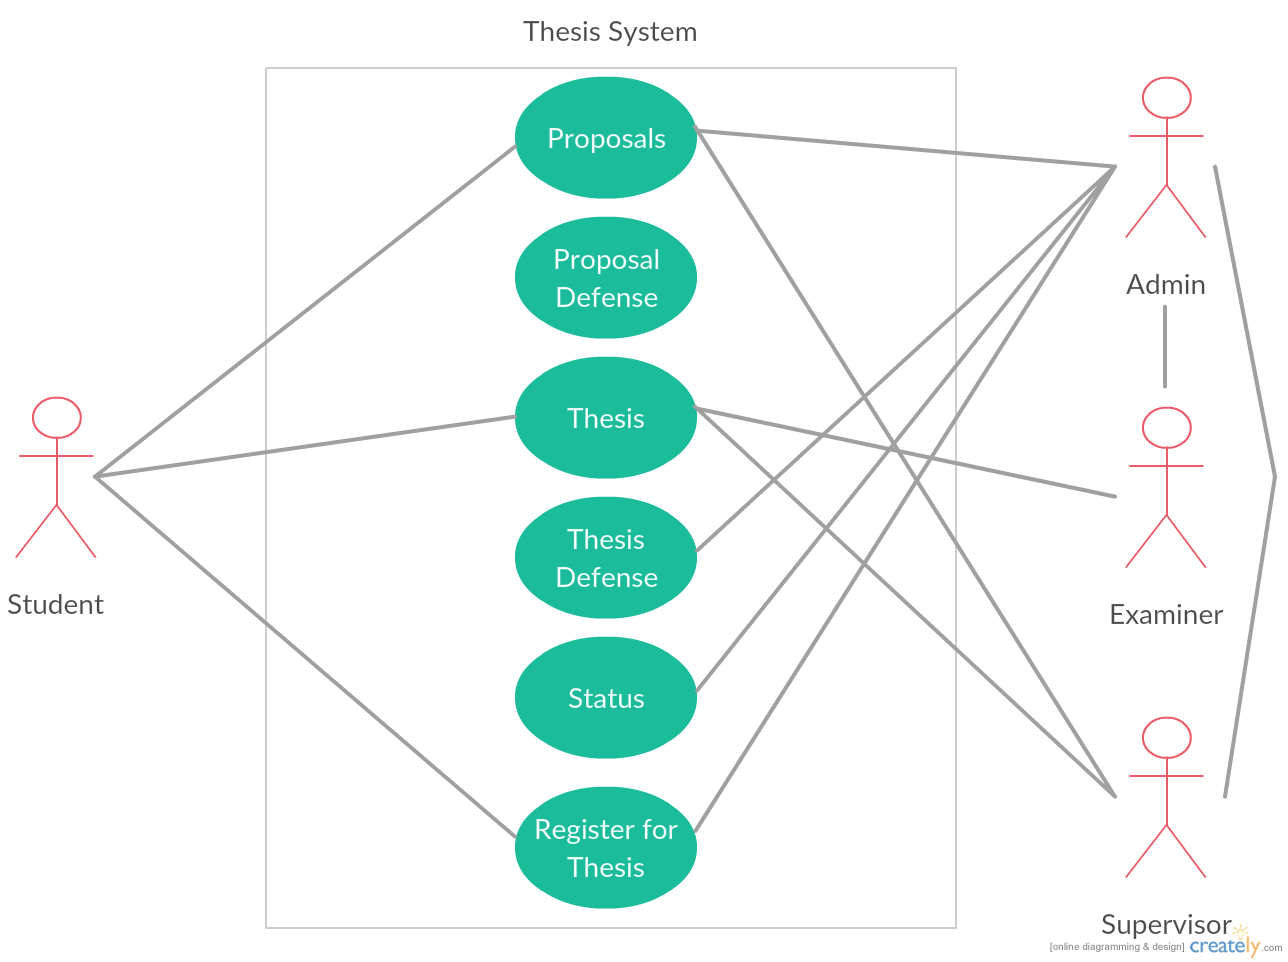
\includegraphics[scale=0.2]{UsecaseDiagram}
\caption{Use-Case Diagram}
\label{fig:UsecaseDiagram}
\end{figure}
\par This use-case diagram basically shows the user's interaction with this application that how user interact with this application. Shows different access levels and functionality of application that user interacts with which use-case.

\par This section describes in further detail elements discussed in the Architecture. Typical viewpoints are: 
\begin{enumerate}
	\item   Conceptual View: In Figure \ref{fig:ComponentDiagm} shows the logical functional elements of the system.  Each component represents a similar grouping of functionality.
	\begin{figure}[ht]
\centering
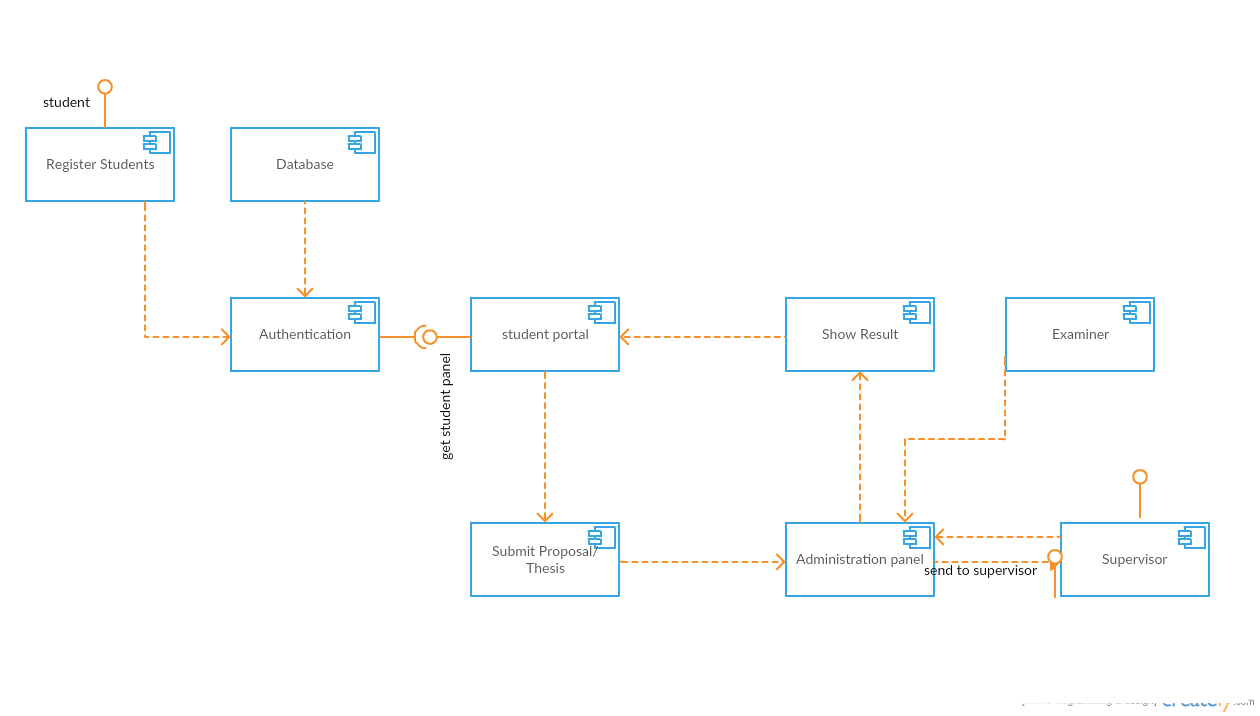
\includegraphics[scale=0.3]{ComponentDiagm}
\caption{Component Diagram}
\label{fig:ComponentDiagm}
\end{figure}

\end{enumerate}
\enlargethispage{-\baselineskip}
\section{Low Level Design}

\par Low level design of the application shows the different layers and shows at which layer which type of operation is perform. Data layer describes which type of data is used, Data access layer describes how data is accessed, Service layer illustrate the service provided to ADD, Business layer shows the complete operation performed by ADD and the last presentation layer illustrate the user interaction with ADD and different user interfaces.

\section{GUI Design}
The GUI of a system requires to be simple and user friendly. Since our designed system will be used by students and faculty members instead of computer scientist, therefore the GUI had to be very user friendly but extremely comprehensive. The best thing about our GUI design is that that it guides the user through step by step by going one activity to another activity. This chapter will explain the graphical user interface of the system. As the core objective of this system is to be used. So we need to design it simple, relevant and user friendly. By taking advantage of an individual suggestions impression, I am designing graphical user interface quite simple yet appealing. All of us use linear page layout for most styles as well as appropriate page layout.
\begin{figure}[ht]
\centering
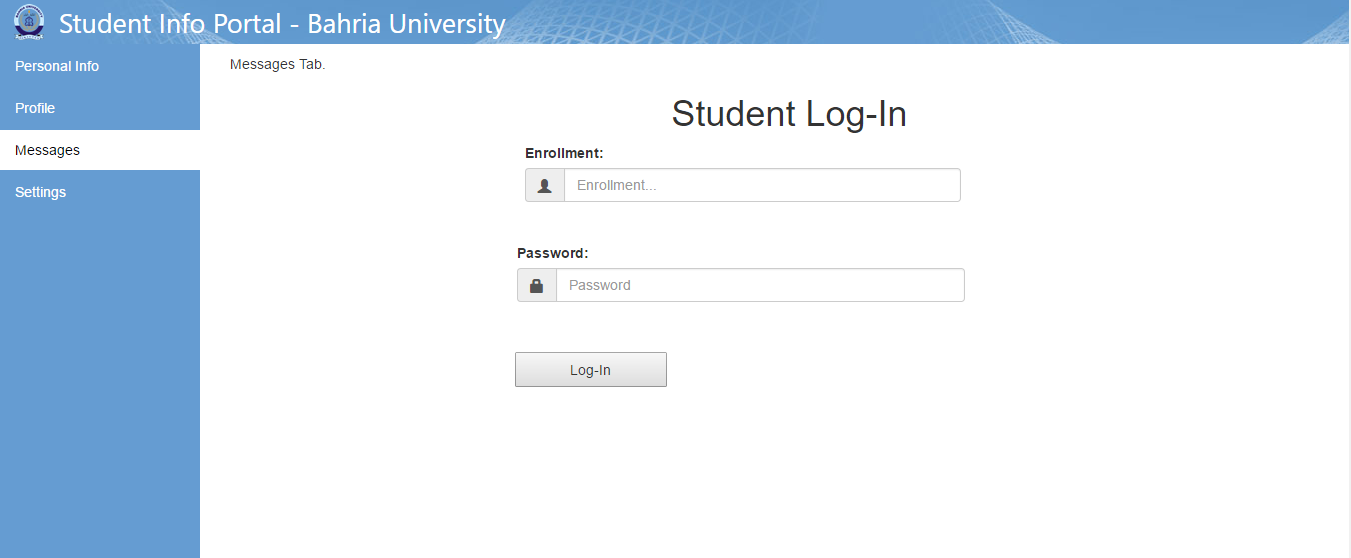
\includegraphics[scale=0.5]{first}
\caption{First User Interface}
\label{fig:first}
\end{figure}




%%\chapter{Chapter 8 title} \label{chap:concl}
%\version{v1.10.2015}
\section*{}
\lipsum

\section{Sec}
\lipsum
%%\printindex
%% comment next 2 commands if numbered appendixes not used
\appendix
\include{appendix1}
%%\chapter{Appendix} \label{ap:appendix2}

\section*{}


%%----------------------------------------
%% Final materials
%%----------------------------------------

\begin{singlespace}
  %% Bibliography
  %% comment the next command if BibTeX file not used
  %% bibliography is in ``references.bib''
  \PrintBib{references}
  Essays, UK. (November 2013). Literature Review About Management Information Systems Management Essay?utm_expid=309629 42.KXZ6CCs5RRCgVDyVYVWeng.0&utm_referrer=https%3A%2F%2Fwww.google.com.pk%2F. Retrieved from https://www.ukessays.com/essays/management/literature-review-about-management-information-systems-management-essay.php?utm_expid=309629-42.KXZ6CCs5RRCgVDyVYVWeng.0&utm_referrer=https%3A%2F%2Fwww.google.com.pk%2F?cref=1

  %% Index
  %% uncomment next command if index is required
  %% don't forget to run ``makeindex tese'' command
  \PrintIndex
\end{singlespace}

\end{document}